\section{RAVEN}
\label{sec:raven}
 
The Risk Analysis and Virtual ENviroment 
(RAVEN
\footnote{Official website: \url{https://raven.inl.gov},\\ 
GITHUB repository: \url{https://github.com/idaholab/raven}})
~\cite{RAVEN_PSAM_2014,alfonsiEsrel2014} 
is a flexible and multi-purpose uncertainty quantification, regression analysis, probabilistic
risk assessment, data analysis and model optimization framework. Depending on the tasks to be 
accomplished and on the probabilistic characterization of the problem, RAVEN perturbs 
(e.g., Monte-Carlo, latin hypercube, reliability surface search) the response of the system 
under consideration by altering its own parameters. The system is modeled by third party software 
(e.g., RELAP5-3D~\cite{relap5}, MELCOR~\cite{Melcor}) and accessible to RAVEN either directly (software coupling) 
or indirectly (via input/output files). The data generated by the sampling process is analyzed using 
classical statistical and more advanced data mining approaches. RAVEN also manages the parallel dispatching 
(i.e. both on desktop/workstation and large High Performance Computing machines) of the software 
representing the physical model. RAVEN heavily relies on artificial intelligence algorithms to construct 
surrogate models of complex physical systems in order to perform uncertainty quantification, reliability 
analysis (limit state surface) and parametric studies.

By statistical analysis we include:
\begin{itemize}
  \item Sampling of codes, either stochastic (e.g., Monte-Carlo~\cite{DynamicReliabilityMonteCarlo} 
        and Latin Hypercube Sampling~\cite{LHShelton}, deterministic (e.g., grid and
        Dynamic Event Tree~\cite{AMENDOLAdylam,cojazziDylam}) or adaptive~\cite{ANS_S_2014_raven_LS,mandelliSVMANS}
  \item Generation of Reduced Order Models (ROMs)~\cite{ROM_Khalik}, also known as Surrogate models
  \item Post-processing of the sampled data and generation of statistical parameters (e.g., mean, 
        variance, covariance matrix).
\end{itemize}

Figure~\ref{fig:ravenScheme} shows a general overview of the elements that comprise the RAVEN statistical framework:

\begin{itemize}
  \item Model: it represents the pipeline between input and output space. It comprises both codes 
        (e.g., RELAP5-3D~\cite{relap5}) and also ROMs 
  \item Sampler: it is the driver for any specific sampling strategy (e.g., Monte-Carlo, LHS, 
        DET~\cite{ANS2014_adaptDET,PSA2013_Raven})
  \item Database: the data storing entity
  \item Post-processing module: the module that performs statistical analyses and visualizes results.
\end{itemize}

\begin{figure}
    \centering
    \centerline{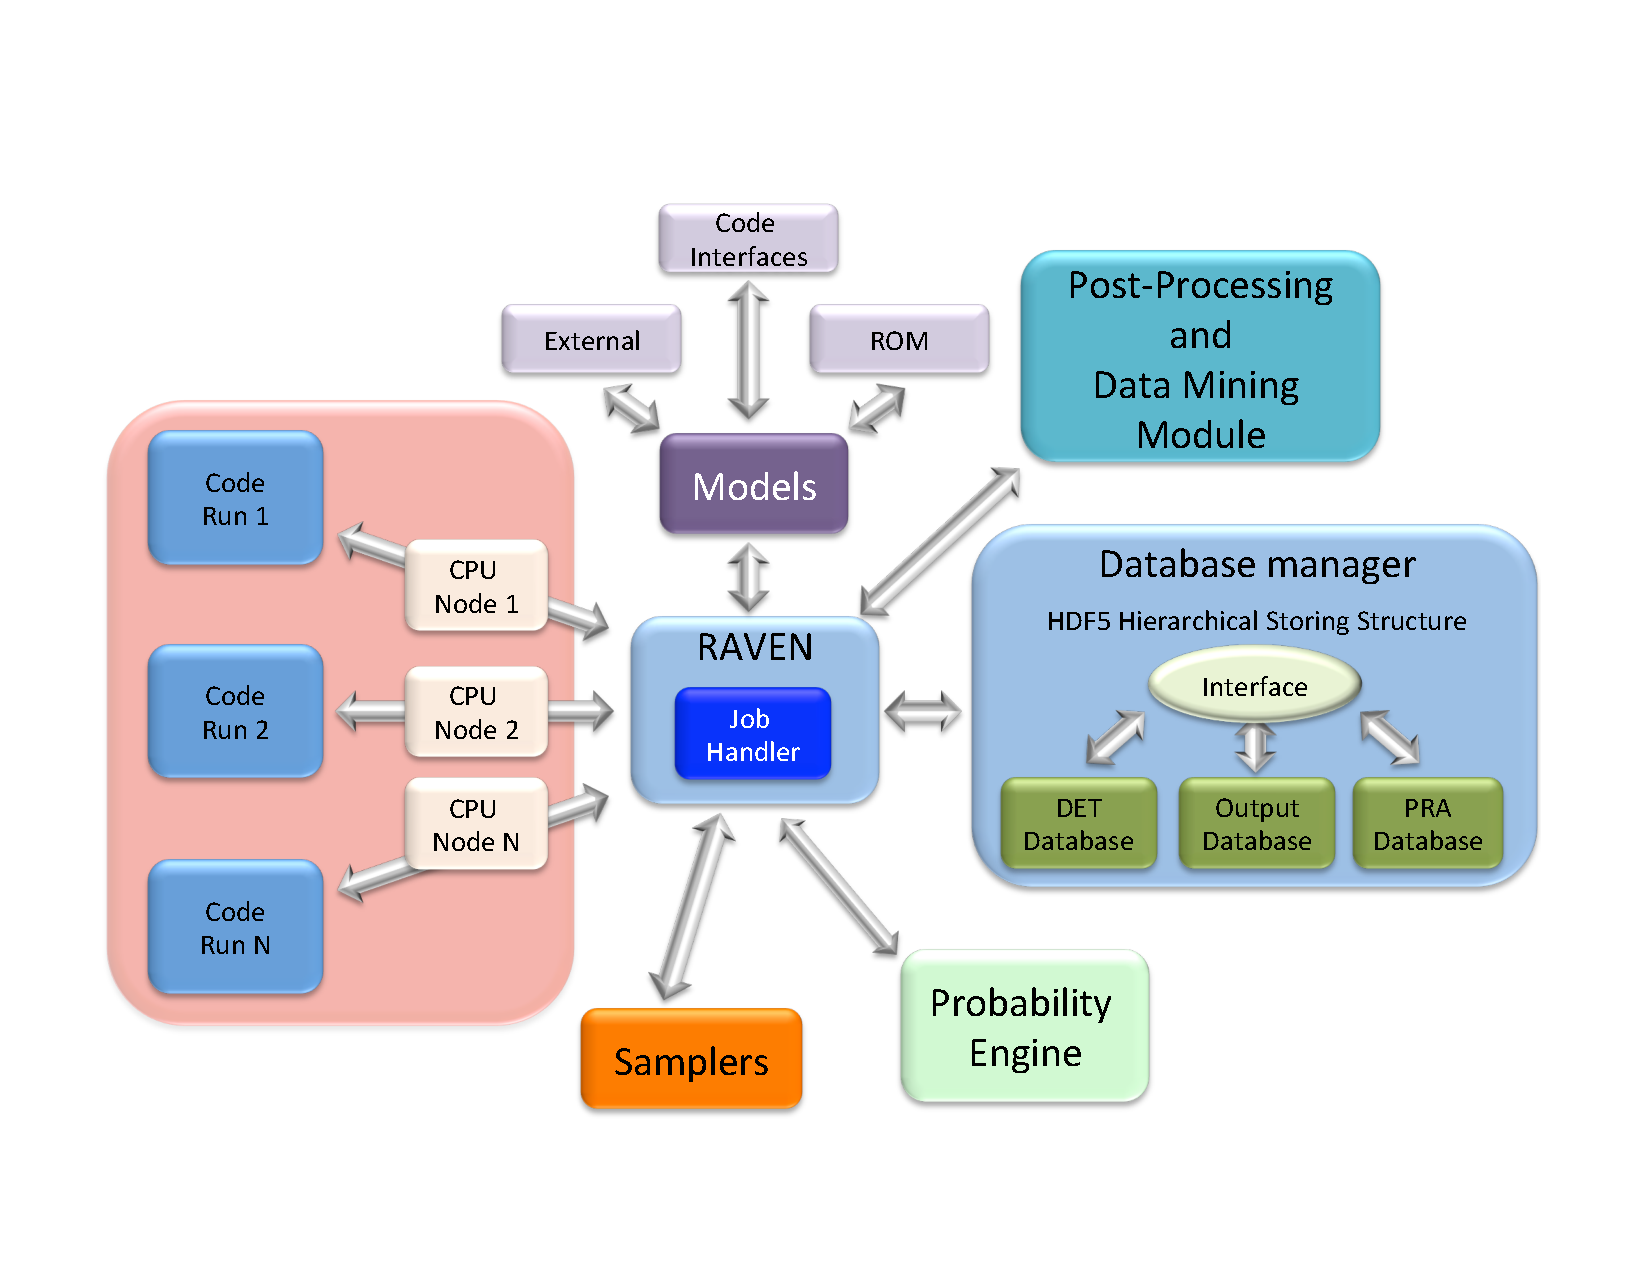
\includegraphics[scale=0.6]{raven.pdf}} 
    \caption{Overview of RAVEN statistical framework components}
    \label{fig:ravenScheme}
\end{figure}

\subsection{Ensemble-Model Capabilities}
[ANDREA]